Como se describió previamente en los objetivos, el desarrollo del presente trabajo puede dividirse en tres partes:
\begin{enumerate}
    \item La implementación del algoritmo seleccionado, \emph{Square Decomposition}.
    \item La herramienta que permite visualizar y modificar los valores de la ejecución de dicho algoritmo.
    \item Las pruebas funcionales del algoritmo.
\end{enumerate}

Debido a ello, este capítulo estará dividida en tres partes, cada una correspondiente a un objetivo.

En cada parte se desarrolla el trabajo realizado para cumplir dicho objetivo, las tecnologías utilizadas para su implementación, se comentará en detalle algunas partes que pueden ser más interesantes y, en el caso de las pruebas, los resultados obtenidos.

Toda la implementación correspondiente a las tres partes puede encontrarse en GitHub en el siguiente enlace: \href{https://github.com/pedrors99/TFG}{https://github.com/pedrors99/TFG}, así como este propio documento.

\section{Implementación de \emph{Square Decomposition}}

En esta parte se estudia cómo queda la implementación del algoritmo en el que se decidió centrar este trabajo, \emph{Square Decomposition}, así como el lenguaje utilizado para su implementación, los distintos archivos y bibliotecas utilizadas y se entrará en detalle en los detalles más interesantes de la implementación.

\subsection{Bibliotecas}

El algoritmo ha sido implementado utilizando \emph{Python 3.11}, además de las siguientes bibliotecas:
\begin{itemize}
    \item \emph{numpy}: Utilizada para almacenar los vectores con los distintos valores utilizados en el Algoritmo extendido de Euclídes en el cálculo de inversos en un anillo.

    \item \emph{random}: Utilizada para la generación aleatoria requerida por \emph{Square Decomposition}. Es debido a esta aleatoriedad proporcionada por \emph{random} que dos ejecuciones distintas nos darán resultados distintos.

    \item \emph{math}: Utilizada para el cálculo de raíces cuadradas.

    \item \emph{dataclasses}: Utilizada para crear objetos similares a los \emph{struct} de otros lenguajes, que son classes con valores pero sin funciones. Estas estructuras servirán para representar los parámetros y las pruebas de los distintos algoritmos.
\end{itemize}

\subsection{Implementación}

Finalmente, se desarrolla cómo está implementado cada uno de los algoritmos. Como fue comentado previamente, cada fichero contiene la implementación tanto del algoritmo que genera la prueba como de su verificación, además de variantes de estas funciones que devuelven un diccionario con valores que normalmente son secretos para poder visualizarlos desde la herramienta. Debido a que el funcionamiento de estas variantes es básicamente el mismo, únicamente se entrará en detalles en uno de ellos para ver esta funcionalidad extra.

Para las pruebas y verificaciones se incluye un parámetro de entrada adicional, \textit{debug}, que es una variable \textit{booleana} por defecto en \textit{False} que determina si imprimir los datos relacionados con el algoritmo, que incluye tanto la entrada, la salida, y algunos de los valores intermedios que utiliza, por pantalla.

\subsubsection{Funciones adicionales}

La mayoría de funciones implementadas son para las pruebas o las verificaciones de las mismas. Sin embargo, hay una serie de funciones adicionales implementadas en los ficheros \emph{utils.py} y \emph{mod.py}.

El primero, \emph{utils.py}, contiene las dos siguientes funciones:
\begin{itemize}
    \item \textit{Hash}: Implementa la función \emph{Hash} utilizada en el algoritmo. Por defecto, como se comentó previamente, será la identidad, es decir, una función tal que:
    $$\operatorname{Hash}(x) = x \hspace{1cm} \forall x$$

    Esto se debe a que se prefiere utilizar una función más simple que permite seguir facilmente el funcionamiento del algoritmo con mayor facilidad.

    \item \textit{concat}: Concatena dos números que se le pasan como parámetros. La salida es el número resultante de dicha concatenación.
\end{itemize}

El segundo de ellos, \emph{mod.py}, contiene una clase que representa un anillo módulo, formada por el valor del número y el valor del módulo. Contiene las funciones necesarias para poder realizar las operaciones básicas, como son la suma, resta, producto, potencias y comparación, así como el cálculo de inversos utilizando el algoritmo extendido de Euclides.

El constructor de esta clase es el siguiente:
\begin{lstlisting}[language=Python, basicstyle=\footnotesize]
class Mod:
    def __init__(self, x, p):
        self.x = x % p
        self.p = p
\end{lstlisting}

Para la mayoría de funciones para las operaciones, como son similares, sólo se mostrará una de ellas, la suma, que servirá como ejemplo:
\begin{lstlisting}[language=Python, basicstyle=\footnotesize]
    def __add__(self, y):
        if isinstance(y, int):
            return Mod(self.x + y, self.p)
        if isinstance(y, Mod):
            assert(self.p == y.p)
            return Mod((self.x + y.x), self.p)
        else:
            self.assertFalse(True)
\end{lstlisting}
Estas funciones permiten tanto operar con otros objetos de esta misma clase, o con enteros.

Finalmente, se representan las dos funciones más complejas en detalle, que son las que se usan para el cálculo de inversos y para las potencias. La primera de ellas se basa en el algoritmo extendido de Euclides, y queda de la siguiente forma:
\begin{lstlisting}[language=Python, basicstyle=\footnotesize]
        def inverse(self):
        if self.x != 0:
            q = np.empty(0)
            r = np.array([self.p, self.x])
            u = np.array([1, 0])
            v = np.array([0, 1])

            while True:
                q = np.append(q, int(r[len(r) - 2] / r[len(r) - 1]))
                r = np.append(r, int(r[len(r) - 2] % r[len(r) - 1]))
                if r[len(r)-1] == 0:
                    break
                u = np.append(u, int(u[len(u)-2] - q[len(q)-1] * u[len(u)-1]))
                v = np.append(v, int(v[len(v)-2] - q[len(q)-1] * v[len(v)-1]))

            assert(r[len(r)-2] == 1), "Error al calcular el inverso de {}".format(self)
            return Mod(v[len(v)-1], self.p)
        else:
            return self
\end{lstlisting}

Para las potencias, tenemos tres casos:
\begin{enumerate}
    \item El exponente es 0. Entonces simplemente se devuelve 1 en el módulo correspondiente.

    \item El exponente es positivo. En este caso, se descompone la potencia como una serie de multiplicaciones, y se le aplica el módulo tras cada multiplicación. Esto, aunque no es muy eficiente en tiempo, evita que se alcancen valores demasiados altos que causen errores. Para optimizar el tiempo, usamos las siguiente propiedad: Si queremos calcular $a^{b} (\operatorname{mod} \text{ p})$ y sabemos que $a^{c} (\operatorname{mod} \text{ p}) = 1$ con $c < b$, entonces podemos simplemente calcular $a^{b \% c} (\operatorname{mod} \text{ p})$, donde $b \% c$ es el resto de dividir $b$ entre $c$.

    \item El exponente es negativo. Como $a^{-b} (\operatorname{mod} \text{ p})$ con $b \in \mathbb{Z}^{+}$, es equivalente calcular $(a^{-1})^{b} (\operatorname{mod} \text{ p})$, donde $a^{-1}$ es el inverso de $a$ en $\mathbb{Z}_{p}$, simplemente calculamos la potencia de su inverso con el exponente positivo.
\end{enumerate}

Nótese que el cálculo de inversos sólo es posible si el valor $x$ y el módulo $p$ son primos relativos. En caso de que no lo sean, se detendrá la ejecución informando del error. Es por ello que se recomienda utilizar como valor para el módulo un número primo o al menos lo menos descomponible posible.

Todo esto queda implementado en la siguiente función:
\begin{lstlisting}[language=Python, basicstyle=\footnotesize]
   def __pow__(self, n):
        if self.x == 0 or self.x == 1:
            return Mod(self.x, self.p)
        else:
            if n == 0:
                return Mod(1, self.p)
            elif n < 0:
                self.x = self.inverse().x
                n = -n

            value = self.x

            for i in range(1, n):
                self.x = (self.x * value) % self.p
                if self.x == 1:
                    return Mod(value, self.p) ** (n % (i+1))

            return Mod(self.x, self.p)
            return self
\end{lstlisting}

\subsubsection{Esquema}

Para que sea más fácil entender que relación entre los distintos algoritmos, se incluyen unas imágenes que contienen los distintos algoritmos y cómo se llaman entre ellos.

Para la prueba de la Descomposición Cuadrada, el esquema es el siguiente: \\
\begin{figure}[H]
    \centering
    \fbox{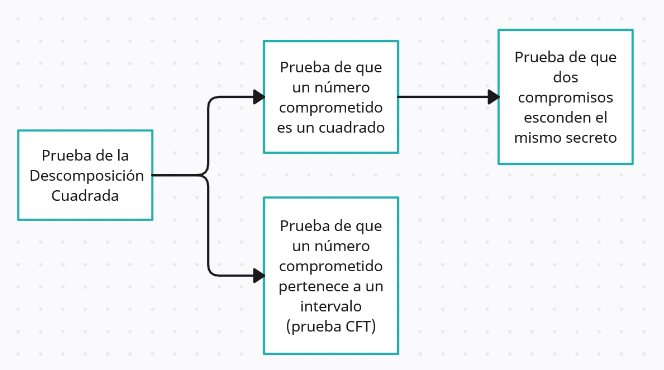
\includegraphics[width=0.75\linewidth]{images/Esquema Prueba.png}}
    \caption{Esquema de la prueba}
\end{figure}

Y análogamente, el de la verificación es: \\
\begin{figure}[H]
    \centering
    \fbox{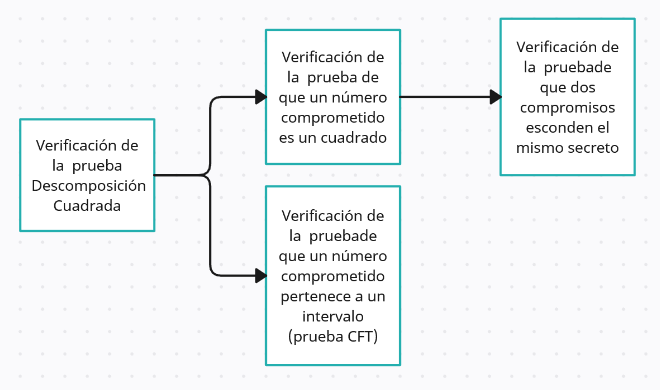
\includegraphics[width=0.75\linewidth]{images/Esquema Verificacion.png}}
    \caption{Esquema de la verificación}
\end{figure}

\subsubsection{Prueba de que dos compromisos esconden el mismo secreto}

Primero se presenta la implementación del algoritmo para la \nameref{proof:ss}, que queda implementada en el fichero \emph{same\_secret.py}. Utiliza dos estructuras, una para los parámetros y otra para la prueba, que son las siguientes:
\begin{lstlisting}[language=Python, basicstyle=\footnotesize]
@dataclass
class paramsSS:
    t: int
    l: int
    s1: int
    s2: int


@dataclass
class proofSS:
    c: int
    D: int
    D1: int
    D2: int
\end{lstlisting}
Se puede ver que todos los parámetros de ambas estructuras son enteros. Este algoritmo se diferencia de los demás ya que es el único que utiliza cuatro parámetros de seguridad: $t, \ell, s1$ y $s2$; mientras que los demás utilizan $t, \ell$ y $s$. Esto se debe a que cada uno de los parámetros $s1$ y $s2$ se utiliza para cada uno de los compromisos. Como se verá más adelante, dentro del algoritmo de \emph{Square Decomposition} inicializamos ambos parámetros con el mismo valor, el de $s$, ya que ambos compromisos pertenecerán al mismo intervalo.

Recordemos que el algoritmo para dicha prueba era el siguiente: \\
\begin{minipage}{0.9\textwidth}
    \begin{algorithm}[H]
        \caption{Prueba del mismo secreto: $\operatorname{Prove_{SS}}$}
        \KwIn{$x, r_{1}, r_{2}, g_{1}, g_{2}, h_{1}, h_{2}, F, \operatorname{params_{SS}}$}
        \KwOut{$\operatorname{proof_{SS}}$}

        $w \in_{R} [1, 2^{\ell+t}b-1]$ \\
        $\upeta_{1} \in_{R} [1, 2^{\ell+t+s_{1}}n-1]$ \\
        $\upeta_{2} \in_{R} [1, 2^{\ell+t+s_{2}}n-1]$ \\
        $\Omega_{1} = g_{1}^{w}h_{1}^{\upeta_{1}} (\operatorname{mod} n)$ \\
        $\Omega_{2} = g_{2}^{w}h_{2}^{\upeta_{2}} (\operatorname{mod} n)$ \\
        $c = \operatorname{Hash}(\Omega_{1} || \Omega_{2})$ \\
        $D = w + cx$ \\
        $D_{1} = \upeta_{1} + cr_{1}$ \\
        $D_{2} = \upeta_{2} + cr_{2}$ \\

        \Return{$\operatorname{proof_{SS}} = (c, D, D_{1}, D_{2})$}
    \end{algorithm}
\end{minipage}

La implementación es la siguiente:
\begin{lstlisting}[language=Python, basicstyle=\footnotesize]
def proveSS(x, n, r1, r2, g1, g2, h1, h2, b, params, debug=False):
    w = random.randint(1, 2 ** (params.l + params.t) * b - 1)
    eta1 = random.randint(1, 2 ** (params.l + params.t + params.s1) * n - 1)
    eta2 = random.randint(1, 2 ** (params.l + params.t + params.s2) * n - 1)
    omega1 = (Mod(g1, n) ** w * Mod(h1, n) ** eta1).x
    omega2 = (Mod(g2, n) ** w * Mod(h2, n) ** eta2).x
    c = utils.hash(utils.concat(omega1, omega2))
    D = w + c * x
    D1 = eta1 + c * r1
    D2 = eta2 + c * r2

    return proofSS(c, D, D1, D2)
\end{lstlisting}

Todas las variables aleatorias se generan utilizando la función \textit{random.randint}, que genera un valor entero aleatorio a partir de los dos parámetros que se le pasen, que funcionan como límites para el intervalo al cuál pertenecerá el valor generado, con ambos extremos incluidos.

Como se comentó previamente, el algoritmo utiliza la clase \textit{Mod} para las operaciones que requieren módulo, pasándole como argumentos el valor y el módulo. Además, en los casos que lo usa, para $\Omega_{1}$ y $\Omega_{2}$ se queda únicamente con $x$, que es el valor ignorando el módulo. Esto se debe a que las siguientes operaciones en las que se utilizan no usaran el módulo.

Por último, se puede ver que la función \textit{utils.concat} se utiliza para, como vimos en la explicación de los ficheros, concatenar dos enteros, es decir:
$$\operatorname{utils.concat(x, y)} = x||y = xy$$
y la función \textit{utils.hash} que, para facilitar el ejemplo, en nuestro caso funciona como la función identidad.

La verificación de la prueba tomará como entrada los parámetros $E$ y $F$, que son los que la prueba quiere demostrar que esconden el mismo secreto, y junto con la prueba y algunos otros parámetros comprueba la veracidad de dicha prueba de la siguiente forma: \\
\begin{minipage}{0.9\textwidth}
    \begin{algorithm}[H]
        \caption{Prueba del mismo secreto: $\operatorname{Verify_{SS}}$}
        \KwIn{$E, F, n, g1, g2, h1, h2, \operatorname{proof_{SS}}$}
        \KwOut{True o False}
        \uIf{$c == \operatorname{Hash}(g_{1}^{D}h_{1}^{D_{1}}E^{-c} (\operatorname{mod} n) || g_{2}^{D}h_{2}^{D_{2}}F^{-c} (\operatorname{mod} n))$}{
            \Return{True}
        } \Else{
            \Return{False}
        }
    \end{algorithm}
\end{minipage}

Esto queda implementada de la siguiente forma:
\begin{lstlisting}[language=Python, basicstyle=\footnotesize]
def verifySS(E, F, n, g1, g2, h1, h2, proof, debug=False):
    val1 = Mod(g1, n) ** proof.D * Mod(h1, n) ** proof.D1 * Mod(E, n) ** (-proof.c)
    val2 = Mod(g2, n) ** proof.D * Mod(h2, n) ** proof.D2 * Mod(F, n) ** (-proof.c)

    return utils.hash(utils.concat(val1.x, val2.x)) == proof.c
\end{lstlisting}

La única diferencia es que dividimos el \textit{if} en los dos cálculos para evitar tener una línea demasiado larga y difícil de comprender, y que en lugar de utilizar una estructura \textit{if/else}, decidimos directamente devolver la igualdad, ya que el resultado es el mismo.

\subsubsection{Prueba de que un número comprometido es un cuadrado}

Similar al algoritmo de la prueba anterior, para la \nameref{proof:s}, que queda implementada en el fichero \emph{square.py}, se utilizan estructuras para los parámetros y para la prueba, que son las siguientes:
\begin{lstlisting}[language=Python, basicstyle=\footnotesize]
@dataclass
class paramsS:
    t: int
    l: int
    s: int


@dataclass
class proofS:
    E: int
    F: int
    proof_ss: proveSS
\end{lstlisting}

Para este algoritmo, los parámetros de seguridad son diferentes, utilizando sólo tres variables, $t, \ell$ y $s$ en lugar de los cuatro del algoritmo anterior, $t, \ell, s_{1}$ y $s_{2}$. En este caso, la prueba incluye un parámetro \textit{proof\_ss} que es la estructura utilizada para la prueba de algoritmo anterior.

El algoritmo de esta prueba era el siguiente: \\
\begin{minipage}{0.9\textwidth}
    \begin{algorithm}[H]
        \caption{Prueba de Cuadrado: $\operatorname{Prove_{S}}$}
        \KwIn{$x, n, E, r_{1}, g, h, b, \operatorname{params_{S}}$}
        \KwOut{$\operatorname{proof_{S}}$}

        $r_{2} \in_{R} [-2^{s}n+1, 2^{s}n-1]$ \\
        $F = g^{x}h^{r_{2}} (\operatorname{mod} \text{ n})$ \\
        $r_{3} = r_{1} - r_{2}x$ \\
        $\operatorname{proof_{ss}} = \operatorname{Prove_{SS}}(x, r_{2}, r_{3}, E, F)$ \\

        \Return{$\operatorname{proof_{S}} = (E, F, \operatorname{proof_{ss}})$}
    \end{algorithm}
\end{minipage} \\
que queda implementado:
\begin{lstlisting}[language=Python, basicstyle=\footnotesize]
def proveS(x, n, E, r1, g, h, b, params, debug=False):
    r2 = random.randint(-2 ** params.s * n + 1, 2 ** params.s * n - 1)
    F = (Mod(g, n) ** x * Mod(h, n) ** r2).x
    r3 = r1 - r2 * x
    params_ss = paramsSS(params.t, params.l, params.s, params.s)

    proof = proveSS(x, n, r3, r2, F, g, h, h, b, params_ss, debug)
    return proofS(E, F, proof)
\end{lstlisting}
donde \textit{proveSS} es el algoritmo de la prueba anterior, la \nameref{proof:ss}.

La única diferencia es la inicialización de los parámetros de seguridad, ya que como hemos comentado, \textbf{proveSS} y \textbf{proveS} no utilizan los mismos.

Este algoritmo nos dará como salida los valores de la prueba, que se le pasará a la verificación junto con algunos otros parámetros, y comprobará si es válida con el siguiente algoritmo: \\
\begin{minipage}{0.9\textwidth}
    \begin{algorithm}[H]
        \caption{Prueba de Cuadrado: $\operatorname{Verify_{S}}$}
        \KwIn{$n, g, h, \operatorname{proof_{S}}$}
        \KwOut{True o False}
        \Return{$\operatorname{Verify_{SS}} (E, F, n, F, g, h, h, \operatorname{proof_{ss}})$}
    \end{algorithm}
\end{minipage} \\
y es implementado de la siguiente forma:
\begin{lstlisting}[language=Python, basicstyle=\footnotesize]
def verifyS(n, g, h, proof, debug=False):
    return verifySS(proof.E, proof.F, n, proof.F, g, h, h, proof.proof_ss, debug)
\end{lstlisting}

Podemos ver que tanto la función de la prueba como de la verificación, al utilizar el algoritmo de la \nameref{proof:ss}, pasan el valor del parámetro \textit{debug}, por lo que en caso de querer comprobar su funcionamiento interno o solucionar algún error, veremos los valores de ambos algoritmos imprimidos por pantalla.

\subsubsection{Prueba de que un número comprometido pertenece a un intervalo (prueba CFT)}

La \nameref{proof:li} está implementada en el fichero \emph{interval.py}, utiliza nuevamente estructuras para los parámetros y la prueba, que son los siguientes:
\begin{lstlisting}[language=Python, basicstyle=\footnotesize]
@dataclass
class paramsLI:
    t: int
    l: int
    s: int


@dataclass
class proofLI:
    C: int
    D1: int
    D2: int
    c: int
\end{lstlisting}

Una prueba de pertenencia a un intervalo $[b_{1}, b_{2}]$ es una prueba de conocimiento que asegura al verificador que el probador conoce $x$ tal que pertenece a $[B_{1}, B_{2}]$, un intervalo que contiene a $[b_{1}, b_{2}]$. Con estos términos, la tasa de expansión de una prueba de pertenencia a un intervalo es la cantidad $delta = (B_{2} - B_{1})/(b_{2} - b_{1})$.

Recordemos que una prueba de que un número comprometido pertenece a un intervalo es la prueba de que un número $x \in I$ pertenece a $J$, siendo la tasa de expansión $\#J/\#I$ (donde $\#I$ representa el cardinal de $I$) igual a $2^{t+\ell+1}$, tiene el siguiente algoritmo: \\
\begin{minipage}{0.9\textwidth}
    \begin{algorithm}[H]
        \caption{Prueba de intervalo mayor: $\operatorname{Prove_{LI}}$}
        \KwIn{$x, n, g, h, r, b, \operatorname{params_{LI}}$}
        \KwOut{$\operatorname{proof_{LI}}$}

        \While{$D_{1} \notin [cb, 2^{t+\ell}b-1]$}{
            $w \in_{R} [0, 2^{t+\ell}b-1]$ \\
            $\upeta \in_{R} [-2^{t+\ell+s}n+1, 2^{t+\ell+s}n-1]$ \\
            $\Omega = g^{w}h^{\upeta} (\operatorname{mod} \text{ n})$ \\
            $C = \operatorname{Hash}(\Omega)$ \\
            $c = C (\operatorname{mod} 2^{t})$ \\
            $D_{1} = w + xc$ \\
            $D_{2} = \upeta + rc \in \mathbb{Z}$ \\
        }

        \Return{$\operatorname{proof_{LI}} = (C, D_{1}, D_{2})$}
    \end{algorithm}
\end{minipage} \\
Este algoritmo queda implementado en la siguiente función:
\begin{lstlisting}[language=Python, basicstyle=\footnotesize]
def proveLI(x, n, g, h, r, b, params, debug=False):
    loop = True

    while loop:
        w = random.randint(0, int(2 ** (params.t + params.l) * b))
        eta = random.randint(-2 ** (params.t + params.l + params.s) * n + 1, 2 ** (params.t + params.l + params.s) * n - 1)

        omega = (Mod(g, n) ** w * Mod(h, n) ** eta).x
        C = utils.hash(omega)
        c = C % (2 ** params.t)
        D1 = w + x * c
        D2 = eta + r * c

        if c * b <= D1 <= 2 ** (params.t + params.l) * b - 1:
            loop = False

    return proofLI(C, D1, D2, c)
\end{lstlisting}
La principal diferencia entre esta implementación es que, como no tenemos inicializado el valor de $D_{1}$, asumimos que no se cumple la condición $D_{1} \in [cb, 2^{t+\ell}b -1]$ para así entrar en el bucle, y hacemos la comprobación al final de cada iteración, una vez que ya se haya inicializado.

La verificación utiliza esta prueba para la verificación de la siguiente forma: \\
\begin{minipage}{0.9\textwidth}
    \begin{algorithm}[H]
        \caption{Prueba de intervalo mayor: $\operatorname{Verify_{LI}}$}
        \KwIn{$E, n, g, h, b, \operatorname{proof_{LI}}$}
        \KwOut{True o False}
        \uIf{$D_{1} \in [cb, 2^{t+\ell}b-1] \wedge C == \operatorname{Hash}(g^{D_{1}}h^{D_{2}}E^{-c} (\operatorname{mod} \text{ n}))$}{
            \Return{True}
        } \Else{
            \Return{False}
        }
    \end{algorithm}
\end{minipage} \\
que se implementa en la función:
\begin{lstlisting}[language=Python, basicstyle=\footnotesize]
def verifyLI(E, n, g, h, b, proof, params, debug=False):
    cond1 = (proof.c * b <= proof.D1 <= 2 ** (params.t + params.l) * b - 1)
    cond2 = (proof.C == utils.hash((Mod(g, n) ** proof.D1 * Mod(h, n) ** proof.D2 * Mod(E, n) ** (-proof.c)).x))

    return cond1 and cond2
\end{lstlisting}
Al igual que en la verificación de que dos compromisos esconden el mismo secreto, dividimos la condición en dos comprobaciones para mayor claridad del código.

\subsubsection{Descomposición Cuadrada}

Finalmente, se muestra la implementación del algoritmo que se estudia en este trabajo, \nameref{proof:sd}, y que está implementado en \emph{square\_decomposition.py}. También se incluye el ejemplo de las funciones adicionales que comentamos al comienzo de la sección que utilizaremos en la herramienta para visualizar datos extra, tanto para las pruebas como para las verificaciones.

Al igual que las demás pruebas, utiliza estructuras para los parámetros y para las pruebas, que son las siguientes:
\begin{lstlisting}[language=Python, basicstyle=\footnotesize]
@dataclass
class paramsSD:
    t: int
    l: int
    s: int


@dataclass
class proofSD:
    Ea: int
    Eb: int
    Ea1: int
    Ea2: int
    Eb1: int
    Eb2: int
    proof_sa: proofS
    proof_sb: proofS
    proof_lia: proofLI
    proof_lib: proofLI
\end{lstlisting}

El algoritmo final, que incluye las pruebas anteriores, era el siguiente: \\
\begin{minipage}{0.9\textwidth}
    \begin{algorithm}[H]
        \caption{Prueba con tolerancia: $\operatorname{Prove_{WT}}$}
        \KwIn{$x, n, g, h, r, a, b, E$}
        \KwOut{$\operatorname{proof_{WT}}$}

        $E_{a} = \sfrac{E}{g^{a}} (\operatorname{mod} \text{ n})$ \\
        $E_{b} = \sfrac{g^{b}}{E} (\operatorname{mod} \text{ n})$ \\
        $x_{a} = x - a$ \\
        $x_{b} = b - x$ \\
        $x_{a_{1}} = \lfloor \sqrt{x - a} \rfloor$ \\
        $x_{a_{2}} = x_{a} - x_{a_{1}}^{2}$ \\
        $x_{b_{1}} = \lfloor \sqrt{b - x} \rfloor$ \\
        $x_{b_{2}} = x_{b} - x_{b_{1}}^{2}$ \\
        \While{$r_{a_{2}} \notin [-2^{s}n+1, 2^{s}n-1]$}{
            $r_{a_{1}} \in_{R} [-2^{s}n+1, 2^{s}n-1]$ \\
            $r_{a_{2}} = r - r_{a_{1}}$ \\
        }
        Seleccionar $r_{b_{1}}$ y $r_{b_{2}}$ tales que $r_{b_{1}} + r_{b_{2}} = -r$. \\
        $E_{a_{1}} = g^{x^{2}_{a_{1}}}h^{r_{a_{1}}} (\operatorname{mod} \text{ n})$ \\
        $E_{a_{2}} = g^{x_{a_{2}}}h^{r_{a_{2}}} (\operatorname{mod} \text{ n})$ \\
        $E_{b_{1}} = g^{x^{2}_{b_{1}}}h^{r_{b_{1}}} (\operatorname{mod} \text{ n})$ \\
        $E_{b_{2}} = g^{x_{b_{2}}}h^{r_{b_{2}}} (\operatorname{mod} \text{ n})$ \\
        $\operatorname{proof_{S_{a}}} = \operatorname{Prove_{S}}(x_{a_{1}}, r_{a_{1}}, E_{a_{1}})$ \\
        $\operatorname{proof_{S_{b}}} = \operatorname{Prove_{S}}(x_{b_{1}}, r_{b_{1}}, E_{b_{1}})$ \\
        $\operatorname{proof_{LI_{a}}} = \operatorname{Prove_{LI}}(x_{a_{2}}, r_{a_{2}}, E_{a_{2}})$ \\
        $\operatorname{proof_{LI_{b}}} = \operatorname{Prove_{LI}}(x_{b_{2}}, r_{b_{2}}, E_{b_{2}})$ \\

        \Return{$\operatorname{proof_{wt}} = (E_{a_{1}}, E_{a_{2}}, E_{b_{1}}, E_{b_{2}}, \operatorname{proof_{S_{a}}}, \operatorname{proof_{S_{b}}}, \operatorname{proof_{LI_{a}}}, \operatorname{proof_{LI_{b}}})$}
    \end{algorithm}
\end{minipage} \\
queda implementado de la siguiente forma:
\begin{lstlisting}[language=Python, basicstyle=\footnotesize]
def proveSD(x, n, g, h, r, a, b, E, params, debug=False):
    Ea = (Mod(E, n) * (Mod(g, n) ** a).inverse()).x
    Eb = (Mod(g, n) ** b * Mod(E, n).inverse()).x

    xa = x - a
    xb = b - x

    xa1 = math.floor(math.sqrt(x - a))
    xa2 = xa - xa1 ** 2

    xb1 = math.floor(math.sqrt(b - x))
    xb2 = xb - xb1 ** 2

    loop = True
    while loop:
        ra1 = random.randint(-2 ** params.s * n + 1, 2 ** params.s * n - 1)
        ra2 = r - ra1

        if -2 ** params.s * n + 1 < ra2 < 2 ** params.s * n - 1:
            loop = False

    rb1 = random.randint(-abs(r), abs(r))
    rb2 = -r - rb1

    Ea1 = (Mod(g, n) ** (xa1 ** 2) * Mod(h, n) ** ra1).x
    Ea2 = (Mod(g, n) ** xa2 * Mod(h, n) ** ra2).x
    Eb1 = (Mod(g, n) ** (xb1 ** 2) * Mod(h, n) ** rb1).x
    Eb2 = (Mod(g, n) ** xb2 * Mod(h, n) ** rb2).x

    proof_sa = proveS(xa1, n, Ea1, ra1, g, h, b, params)
    proof_sb = proveS(xb1, n, Eb1, rb1, g, h, b, params)

    proof_lia = proveLI(xa2, n, g, h, ra2, b, params)
    proof_lib = proveLI(xb2, n, g, h, rb2, b, params)

    return proofSD(Ea, Eb, Ea1, Ea2, Eb1, Eb2, proof_sa, proof_sb, proof_lia, proof_lib)
\end{lstlisting}

La versión modificada que devuelve parámetros extra es:
\begin{lstlisting}[language=Python, basicstyle=\footnotesize]
def proveSD_Flask(x, n, g, h, r, a, b, E, params, debug=False):
    Ea = (Mod(E, n) * (Mod(g, n) ** a).inverse()).x
    Eb = (Mod(g, n) ** b * Mod(E, n).inverse()).x

    xa = x - a
    xb = b - x

    xa1 = math.floor(math.sqrt(x - a))
    xa2 = xa - xa1 ** 2

    xb1 = math.floor(math.sqrt(b - x))
    xb2 = xb - xb1 ** 2

    loop = True
    while loop:
        ra1 = random.randint(-2 ** params.s * n + 1, 2 ** params.s * n - 1)
        ra2 = r - ra1

        if -2 ** params.s * n + 1 < ra2 < 2 ** params.s * n - 1:
            loop = False

    rb1 = random.randint(-abs(r), abs(r))
    rb2 = -r - rb1

    Ea1 = (Mod(g, n) ** (xa1 ** 2) * Mod(h, n) ** ra1).x
    Ea2 = (Mod(g, n) ** xa2 * Mod(h, n) ** ra2).x
    Eb1 = (Mod(g, n) ** (xb1 ** 2) * Mod(h, n) ** rb1).x
    Eb2 = (Mod(g, n) ** xb2 * Mod(h, n) ** rb2).x

    proof_sa, ext_sa, ext_ssa = proveS_Flask(xa1, n, Ea1, ra1, g, h, b, params)
    proof_sb, ext_sb, ext_ssb = proveS_Flask(xb1, n, Eb1, rb1, g, h, b, params)

    proof_lia, ext_lia = proveLI_Flask(xa2, n, g, h, ra2, b, params)
    proof_lib, ext_lib = proveLI_Flask(xb2, n, g, h, rb2, b, params)

    ext_wt = {'xa': xa, 'xb': xb, 'ra1': ra1, 'ra2': ra2, 'rb1': rb1, 'rb2': rb2, 'xa1': xa1, 'xa2': xa2, 'xb1': xb1,
              'xb2': xb2}

    return proofSD(Ea, Eb, Ea1, Ea2, Eb1, Eb2, proof_sa, proof_sb, proof_lia, proof_lib), ext_wt, ext_sa, ext_ssa,  ext_sb, ext_ssb, ext_lia, ext_lib
\end{lstlisting}
Se puede ver que el funcionamiento es el mismo, pero utilizando las funciones modificadas del resto de pruebas, que nos devuelven diccionarios con los valores adicionales, además de un nuevo diccionario con los valores utilizados en esta prueba.

La verificación utiliza las verificaciones de las pruebas previas para comprobar si la prueba generada por este algoritmo es válida o no. Su algoritmo era: \\
\begin{minipage}{0.9\textwidth}
    \begin{algorithm}[H]
        \caption{Prueba con tolerancia: $\operatorname{Verify_{WT}}$}
        \KwIn{$\operatorname{proof_{WT}}$}
        \KwOut{True o False}
        \If{$E_{a_{2}} == \sfrac{E_{a}}{E_{a_{1}}} (\operatorname{mod} \text{ n}) \wedge E_{b_{2}} == \sfrac{E_{b}}{E_{b_{1}}} (\operatorname{mod} \text{ n})$}{
            $b_{S} = \operatorname{Verify_{S}}(\operatorname{proof_{S_{a}}}) \wedge \operatorname{Verify_{S}}(\operatorname{proof_{S_{b}}})$ \\
            $b_{LI} = \operatorname{Verify_{LI}}(\operatorname{proof_{LI_{a}}}) \wedge \operatorname{Verify_{LI}}(\operatorname{proof_{LI_{b}}})$ \\
            \Return{$b_{S} \wedge b_{LI}$}
        }
        \Return{False}
    \end{algorithm}
\end{minipage} \\
que se implementa de la siguiente forma:
\begin{lstlisting}[language=Python, basicstyle=\footnotesize]
def verifySD(n, g, h, b, proof, params, debug=False):
    if proof.Ea2 == (Mod(proof.Ea, n) * Mod(proof.Ea1, n).inverse()).x and proof.Eb2 == (Mod(proof.Eb, n) * Mod(proof.Eb1, n).inverse()).x:
        bs = verifyS(n, g, h, proof.proof_sa, debug) and verifyS(n, g, h, proof.proof_sb, debug)
        bli = verifyLI(proof.Ea2, n, g, h, b, proof.proof_lia, params, debug) and verifyLI(proof.Eb2, n, g, h, b, proof.proof_lib, params, debug)
        return bs and bli
    else:
        return False
\end{lstlisting}

La versión modificada para mostrar valores adicionales en la herramienta es la siguiente:
\begin{lstlisting}[language=Python, basicstyle=\footnotesize]
def verifySD_Flask(n, g, h, b, proof, params, debug=False):
    cond1 = (proof.Ea2 == (Mod(proof.Ea, n) * Mod(proof.Ea1, n).inverse()).x)
    cond2 = (proof.Eb2 == (Mod(proof.Eb, n) * Mod(proof.Eb1, n).inverse()).x)

    if cond1 and cond2 and proof.Ea1 == proof.proof_sa.E and proof.Eb1 == proof.proof_sb.E:
        cond3 = verifyS(n, g, h, proof.proof_sa, debug)
        cond4 = verifyS(n, g, h, proof.proof_sb, debug)

        cond5 = verifyLI(proof.Ea2, n, g, h, b, proof.proof_lia, params, debug)
        cond6 = verifyLI(proof.Eb2, n, g, h, b, proof.proof_lib, params, debug)

        bs = cond3 and cond4
        bli = cond5 and cond6

        ext = {'cond1': cond1, 'cond2': cond2, 'cond3': cond3, 'cond4': cond4, 'cond5': cond5, 'cond6': cond6}

        return (bs and bli), ext
    else:
        ext = {'cond1': cond1, 'cond2': cond2, 'cond3': '?', 'cond4': '?', 'cond5': '?', 'cond6': '?'}

        return False, ext
\end{lstlisting}

Esta función divide la primera verificación en dos para poder mostrar los resultados de cada una en la herramienta. Además, nuevamente llama a las versiones modificadas de las demás verificaciones. En caso de que falle la primera comprobación, como las demás no se realizan, simplemente devuelve \emph{?} para indicar que el valor es desconocido.

\section{Interfaz de la herramienta}

Para facilitar el entendimiento del funcionamiento del algoritmo, se ofrece una interfaz web que permite visualizar los pasos que sigue el algoritmo, así como los valores y resultados de cada paso. Además, se podrán modificar los valores de entrada y la prueba obtenida para ver cómo modifican los resultados.

Para ello, se implementa una página web utilizando HTML para el Front-End, y la implementación desarrollada en la parte anterior como Back-End, utilizando \emph{Flask} para comunicar el cliente con el servidor. Además, para mejorar el diseño de la página web, utilizaremos Bulma \cite{Bulma}, que nos proporciona clases para los botones y otros elementos que directamente nos proporcionan una mejor apariencia.

Para toda esta implementación, se añade un nuevo fichero a Python:
\begin{itemize}
    \item \emph{flask\_backend.py}: Funciona como servidor, leyendo los valores introducidos por el usuario en la página web, realizando los cálculos con la implementación previa, redirigiendo a las páginas correspondientes y mostrándo los resultados. Consta de una función por cada una de las páginas web.
\end{itemize}

Además, se incluye una carpeta llamada \emph{html} con los distintos archivos utilizados para cada una de las páginas, que son los siguientes:
\begin{itemize}
    \item \emph{input.html}: Es la primera página de la herramienta, en la que aparecen una serie de campos para que se puedan introducir los valores que utilizará el algoritmo. Estos valores están inicializados por defecto para poder realizar la prueba rápidamente, aunque pueden ser modificados a los que se deseen probar.
    
    En la parte inferior encontraremos un botón para continuar, que realizará algunas comprobaciones, como que el intervalo tenga sentido (la cota inferior sea menor que la inferior y ambos valores sean menores que el módulo) y que el secreto pertenece a dicho intervalo. En caso de que haya algún fallo, se avisará indicando como solucionarlo. En caso de que la entrada sea válida, continuará a la siguiente página, \emph{prove\_sd.html}.

    \item \emph{prove\_sd.html}: En esta página se hace un breve resumen del algoritmo \emph{Square Decomposition}, se muestran los valores que toma por entrada, el funcionamiento del algoritmo, y los valores correspondientes a la prueba que se obtienen de salida.

    Además, consta de una sección con botones para redirigir a las pruebas que utiliza el algoritmo internamente, para comprobar que un número comprometido es un cuadrado y para probar que un número comprometido pertenece a un intervalo.

    Finalmente, en la parte inferior de la página tenemos un botón que nos redirigirá a la página anterior, \emph{input.html}, y otro que nos redirigirá a la verificación de la prueba. Esta verificación tomará como entrada los valores que se encuentran en la salida del algoritmo, que pueden ser modificados en caso de que se quiera ver cómo la verificación cambia en caso de que la prueba no sea válida.

    \item \emph{verify\_sd.html}: Esta página contiene los resultados de la verificación, así como los valores que toma de entrada y el funcionamiento de esta verificación. Análogamente a la página anterior, como esta verificación utiliza la verificación de que un número comprometido es un cuadrado y de que un número comprometido pertenece a un intervalo, hay una sección con botones para redirigirnos a las páginas correspondientes.

    Finalmente, también hay un botón en la parte inferior que nos permite volver a la página anterior, \emph{prove\_sd.html}.

    \item \emph{prove\_s.html}: En esta página se muestra el funcionamiento de la prueba de que un número comprometido es un cuadrado, así como los valores que toma como entrada y los que optiene como salida. Análogamente a las páginas anteriores, como esta prueba utiliza la prueba de que dos compromisos esconden el mismo secreto, hay una sección con un botón para redirigirnos a la página de dicha prueba.

    Al igual que \emph{prove\_sd.html}, tiene un botón en la parte inferior de la página que nos redirigirá a la página anterior y otro que nos redigirá a su verificación.

    \item \emph{verify\_s.html}: Similar a \emph{verify\_sd.html}, en esta página se realiza la verificación de la prueba de que un número comprometido es un cuadrado, mostrando los valores de entrada, el algoritmo y el resultado de dicha verificación. Al usar la verificación de que dos compromisos esconden el mismo secreto, constará de una sección con un botón para acceder a la página correspondiente a dicha verificación, \emph{verify\_ss.html}.

    Finalmente, en la parte inferior de la página hay un botón para volver a la página anterior, que puede ser tanto \emph{prove\_s.html} o \emph{verify\_sd.html} dependiendo de la página que hayamos usado para acceder a esta.

    \item \emph{prove\_li.html}: Funcionamiento análogo a \emph{prove\_s.html}, pero con la prueba de que un número comprometido pertenece a un intervalo. Se muestra la entrada, el funcionamiento del algoritmo y el resultado obtenido. Al igual que las demás páginas, tenemos un botón para volver a la página anterior.

    \item \emph{verify\_li.html}: Muestra la verificación de la prueba de que un número comprometido pertenece a un intervalo, incluyendo las entradas de la verificación, su funcionamiento y el resultado obtenido. Además, incluye el botón para volver a la página anterior.

    \item \emph{prove\_ss.html}: Esta página muestra la prueba de que dos compromisos esconden el mismo secreto, detallando los valores de entrada, el algoritmo y la salida.

    Similar a las otras pruebas, consta de un botón para acceder a la página de su verificación, \emph{verify\_ss.html}, y otro botón para volver a la página anterior.

    \item \emph{verify\_ss.html}: Finalmente, en esta última página se muestra la verificación de que dos compromisos esconden el mismo secreto, mostrando la entrada, el funcionamiento y el resultado.
\end{itemize}

Por lo que, en resumen, tenemos una página inicial para las entradas, y una para cada prueba y para cada verificación, disponiendo en todas menos en la página de entrada los valores de entrada, el funcionamiento del algoritmo, la salida y, en caso de que utilice algún otro algoritmo, un botón para acceder a la página correspondiente a dicho algoritmo. Además, las pruebas incluyen botones para acceder a sus verificaciones.

Un resumen de las diversas páginas y las conexiones entre ellas puede verse en el esquema de la \autoref{im:esquema}. En este esquema, una flecha indica que la página señalada es accesible pulsando el botón correspondiente desde la página en la que se origina la flecha. Aunque, como todas las páginas tienen un botón para volver anterior, es posible recorrerlo en el sentido contrario.
\begin{sidewaysfigure}[hbtp]
    \centering
    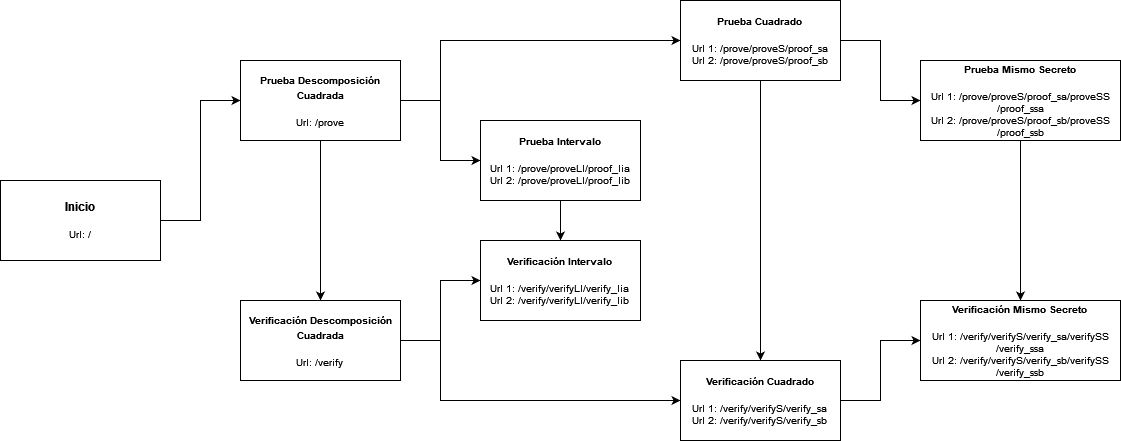
\includegraphics[width=\columnwidth]{images/Esquema.png}
    \caption{Esquema de las páginas web}
    \label{im:esquema}
\end{sidewaysfigure}

Una guía detallada del funcionamiento de esta herramienta con imágenes de las diferentes páginas web puede encontrarse en el \nameref{anexo:html}.

Con todo esto, disponemos de una herramienta que permite ver en detalle el funcionamiento del algoritmo, pudiendo modificar los valores de entrada, viendo los resultados obtenidos en cada paso, y pudiendo modificar las salidas para forzar errores en la verificación.

\section{Verificación del funcionamiento del algoritmo} \label{sec:verificacion}

Finalmente, en esta parte se verifica que el algoritmo funciona tal y como se espera. Esto incluye realizar las dos siguientes comprobaciones:
\begin{enumerate}
    \item Si los valores obtenidos de la prueba son correctos, la verificación debe devolver que es verdadero.

    \item Si los valores obtenidos de la prueba son incorrectos, la verificación debe devolver que es falso.
\end{enumerate}

Además, se va a probar que esto ocurre con distintos valores de entrada, tanto del secreto, como del intervalo, el módulo, los parámetros de seguridad y los generadores. Como extra, se calculan los tiempos de ejecución para ver si existe alguna relación entre estos y el tamaño del módulo.

Para ello, se añade un nuevo fichero a Python, \emph{verification.py}, que es el encargado de realizar las pruebas. Para ello, inicializa un vector de números primos de distinto tamaño que se usa para los módulos de las distintas pruebas, que contiene:
$$[31, 607, 1291, 2053, 2803, 3637, 4481, 5351, 6203, 7057,$$ $$7963, 8867, 9769, 10709, 11699]$$
valores que se han seleccionado de forma aleatoria a partir de una lista de números primos intentando mantener una distancia similar entre ellos.

Luego, para cada uno de los módulos seleccionados se realizan 200 pruebas, para las cuales se seleccionan valores aleatoriamente en las que se asegura que el intervalo es correcto (la cota inferior es menor que la mayor), que el secreto pertenece al intervalo, y que todos estos valores y los generadores son menores que el módulo. Además, también se toman valores aleatorios para los parámetros de seguridad, que estarán entre 1 y 6 (ambos incluidos). Estos valores son mucho más pequeños porque el algoritmo siempre los usa como potencias, y si fueran mucho mas grandes podrían relentizar los cálculos o incluso provocar errores debido a que genera valores demasiado grandes.

Una vez seleccionados los valores, se utiliza el algoritmo para calcular la prueba y verificar que es verdadera y que, por lo tanto, se consigue la comprobación 1 de esta parte ya que con valores obtenidos de la prueba son correctos, la verificación devuelve que es verdadero.

Para la segunda comprobación, se usa una función a la que se le pasan todos los valores de la prueba, y los modificará de manera aleatoria. Esta aleatoriedad incluye el número de valores que modificará (al menos uno), y cómo lo modificará. Una vez modificados, se vuelve a verificar si esta nueva prueba es correcta.

Con todos estos resultados, se puede construir una matriz de confusión, que es una matriz en la que mostramos, de las pruebas verdaderas, cuáles verifica como correctas (verdaderos positivos, o \emph{True Positives}) y cuáles verifica como incorrectas (falsos negativos, o \emph{False Negatives}), y de las pruebas falsas, que hemos modificado, cuáles verifica como correctas (falsos positivos, o \emph{False Positives}) y cuáles verifica como incorrectas (verdaderos negativos, o \emph{True Negatives}). Los resultados que se obtienen para una ejecución son los siguientes:

\begin{figure}[H]
    \centering
    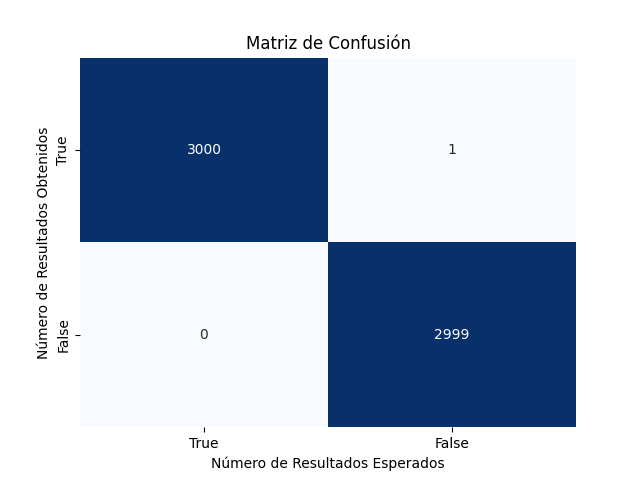
\includegraphics[width=0.75\textwidth]{images/Resultados test.png}
    \caption{Matriz de confusión de los resultados}
\end{figure}

Estos resultados pueden variar debido a la aleatoriedad tanto en la selección de los valores discutidos en esta parte, como en la propia aleatoriedad de los algoritmos. Sin embargo, las pruebas verdaderas siempre las clasifica como verdaderas (es decir, satisface la completitud) y, de las pruebas falsas, casi todas son clasificadas como falsas.

Para comprobarlo, se realizan varias pruebas, y el número de errores que se obtienen en cada una son los de la \autoref{im:resultados}. Esto demuestra que, aunque el número de errores puede variar, suele ser relativamente bajo, normalmente menor o igual a 3. Sabiendo que usa 15 valores distintos para el módulo, que se realizan 200 pruebas para cada uno de los valores y que para cada caso se realiza una prueba verdadera sin modificar y otra modificando los resultados, tenemos un total de 6000 pruebas, por lo que el error es inferior al 0.05\%.

\begin{figure}[H]
    \centering
    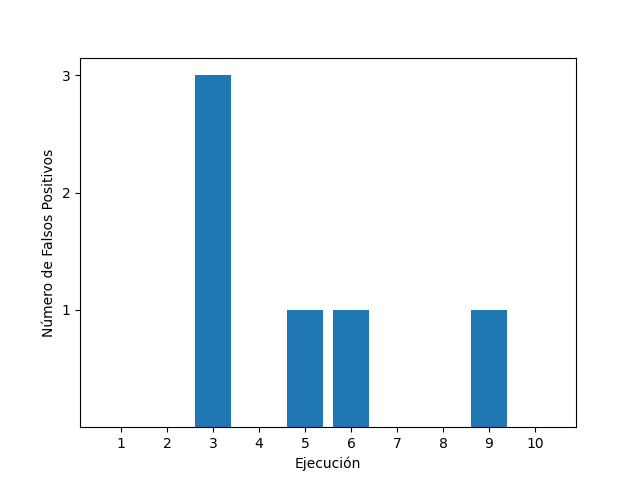
\includegraphics[width=0.75\textwidth]{images/resultados.png}
    \caption{Número de errores}
    \label{im:resultados}
\end{figure}

El hecho de que acepte estas pruebas falsas puede deberse a los siguientes motivos:
\begin{itemize}
    \item Debido a la tolerancia. Como se vió en la prueba de que un número comprometido pertenece a un intervalo, tenemos una pequeña tolerancia, $\theta$, que la verificación aceptaría como correcta sin serlo.

    \item Debido a que la modificación proporciona valores que coincidirían con otra prueba correcta. Esto principalmente ocurre porque, como nuestra intención es mostrar el funcionamiento del algoritmo y, por lo tanto, preferimos tomar valores pequeños que permiten seguir el funcionamiento del algoritmo con mayor facilidad y aceleran los cálculos, hacen que sea más probable que ocurra. Tomando valores más grandes, y modificando la función \emph{Hash} por una más compleja que la identidad, como por ejemplo \emph{md5}, estos casos serán mucho menos probables.
\end{itemize}

Finalmente se comprueba como afecta el tamaño del módulo al tiempo de ejecución. Para ello, se utiliza la biblioteca \emph{time} para guardar el tiempo antes y después de las 200 pruebas con cada uno de los valores seleccionados, y se calcula la media. Esto incluye tanto el tiempo de generar la prueba y verificarla, como el tiempo de modificarla y volver a modificarla. Los tiempos obtenidos se pueden ver en la \autoref{im:tiempos}.

\begin{figure}[ht]
    \centering
    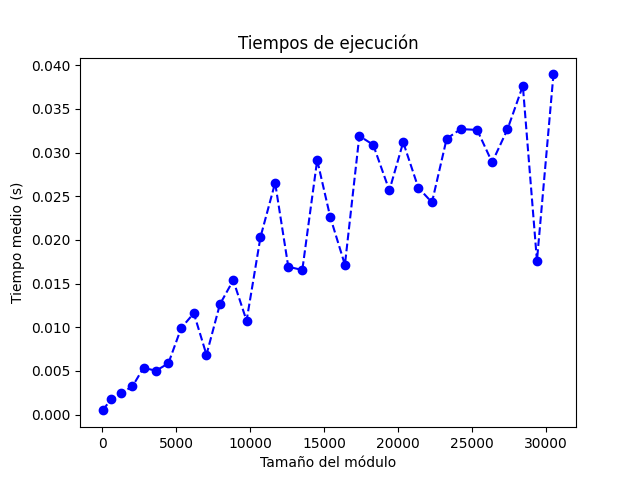
\includegraphics[width=0.75\textwidth]{images/tiempos.png}
    \caption{Tiempos de ejecución con 34 módulos distintos}
    \label{im:tiempos}
\end{figure}

\begin{figure}[ht]
    \centering
    \begin{subfigure}[c]{0.6\textwidth}
        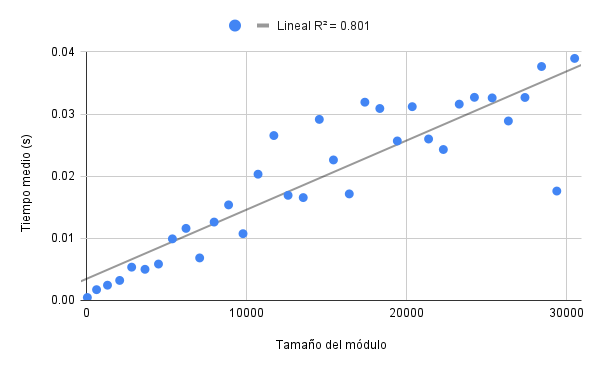
\includegraphics[width=\textwidth]{images/lineal.png}
        \caption{Regresión lineal}
    \end{subfigure}
    \begin{subfigure}[c]{0.6\textwidth}
        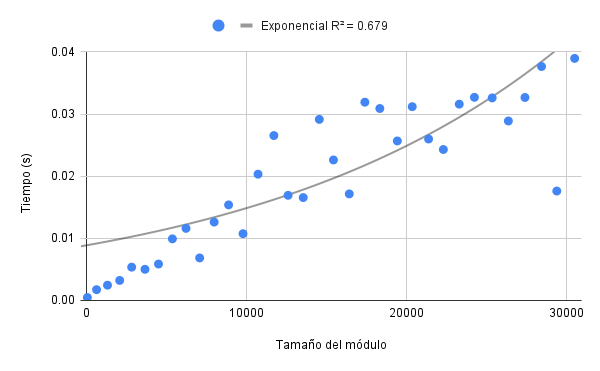
\includegraphics[width=\textwidth]{images/exponencial.png}
        \caption{Regresión exponencial}
    \end{subfigure}
    
    \begin{subfigure}[c]{0.6\textwidth}
        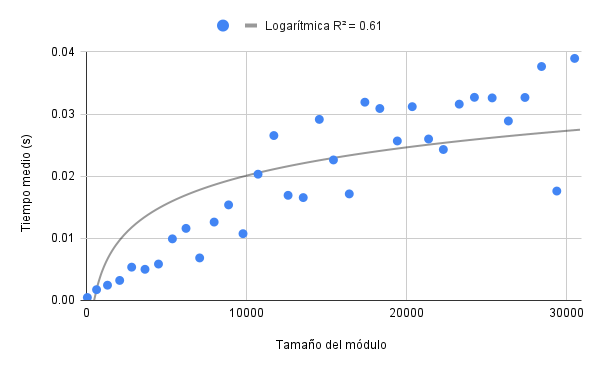
\includegraphics[width=\textwidth]{images/logaritmica.png}
        \caption{Regresión exponencial}
    \end{subfigure}
    \caption{Regresiones lineal, exponencial y logarítmica}
    \label{im:tiempos2}
\end{figure}

En la figura \autoref{im:tiempos2} se puede ver como, al ser mayor $R^{2}$ en el caso lineal, el tiempo aumenta al aumentar el tamaño del módulo de forma aproximadamente lineal, aunque con cierto error debido a la aleatoriedad. Para estas figuras, los módulos seleccionados son:

$$[31, 607, 1291, 2053, 2803, 3637, 4481, 5351, 6203, 7057, 7963, 8867,$$
$$9769, 10709, 11699, 12589, 13537, 14543, 15427, 16417, 17393, 18329, 19423,$$
$$20357, 21379, 22303, 23297, 24247, 25357, 26371, 27409, 28447, 29401, 30517]$$